\chapter{Qualitätssicherung}
\label{chap:Qualitätssicherung}
Die Qualität des Source-To-Source Compilers muss während und nach der erfolgreichen Implementierung sichergestellt werden. In diesem Kapitel werden im ersten Abschnitt die Komponententests als Qualitätsischerungsmaßnahme wärend der Entwicklung thematisiert.  Anschließend wird die Funktionsweise mithilfe einer speziell entwickelten Xamarin.Forms App überprüft.  Anhand dieses Tests kann anschließend überprüft werden, ob  der Compiler erwartungsgemäß funktioniert. 

\section{Komponententests}
Komponententests unterteilen ein Programm in einzelne testfähige Einheiten und validiert deren Funktionalität.  In Visual Studio können diese Testfälle automatisiert ausgeführt werden, wenn Änderungen am Quelltext durchgeführt werden.  Auf diese Weise ist Sichergestellt, dass Änderungen am Quelltext nicht vom gewünschten Verhalten abweichen.  Komponententests optimieren die Qualität des Quelltextes, wenn sie ein integraler Bestandteil des Entwicklungsprozesses sind.  Sobald eine Klasse oder Methode geschrieben ist,  können Komponententests erstellt werden, mit denen das Verhalten des Codes bei der Eingabe von Werten überprüft werden kann.  Klassischerweise werden dafür gültige Daten,  falsche Daten und Daten die an der Grenze des Gültigkeitsbereiches liegen übergeben.  Dieses vorgehen wurde während der Entwicklung des Compilers durchgeführt.  Dieses vorgehen wird häufig als testgesteuerte(engl. testdriven) Entwicklung beschrieben,  bei der die Komponententests vor dem Code geschrieben werden.  Bei diesem Vorgehen dienen die Tests ebenfalls als Entwurfsdokumentation und als funktionale Spezifikationen der Anforderung.



\section{Testobjekt}
Die Testapp wurde mit der Version 5.0.0.2012 des Xamarin.Forms Frameworks realisiert und verwendet die Erweiterungen Xamarin. Essentials.  Das Testobjekt soll möglichst viele Funktionalitäten von Xamarin.Forms abbilden, hat jedoch nicht den Anspruch einer vollständigen Testabdeckung.
Auf plattformspezifische Implementationen mit Ausnahme der Metadaten und Ressourcen wurde verzichtet.  Eine genaue Beschreibung der App-Funktionalitäten und -Eigenschaften folgt und wird mithilfe von iOS Screenshots veranschaulicht.  Die entsprechenden Android Screenshots befinden sich in \hyperref[chap:AnhangAndroidScreenshots]{Anhang III}.

Anhand des Namens,  SampleApp,  und eines Anwendungsicons können Anwender die Benutzer die App auf dem Startbildschirm identifizieren.  Nach dem Start öffnet sich eine Menüstruktur,  die Wurzel der Navigation, über die verschiedene Bereiche der mobilen Anwendung angesteuert werden können.  Abbildung \ref{fig:TestObjectI} zeigt im ersten Screenshoot das Icon und den Namen,  im zweiten das Menu der App und im dritten die Visualisierung der verfügbaren Steuerelemente.

\newpage
\begin{figure}[!ht]
 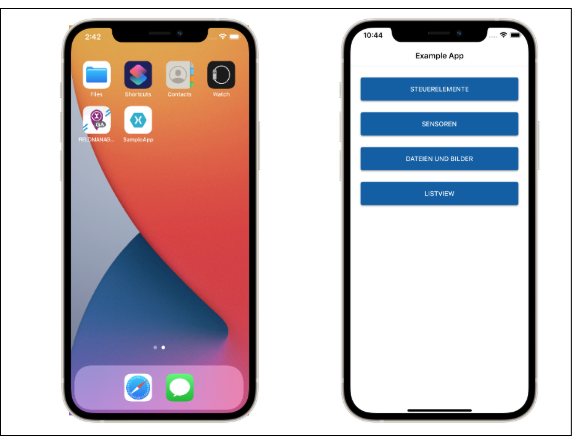
\includegraphics[width=\textwidth,keepaspectratio]{Images/Screenshot/AppIconAndMenu.png}
 \caption{Test Objekt Screenshots I}
 \label{fig:TestObjectI}
\end{figure}
Neben der Navigation zu den Steuerelemente ist es  möglich zu einer Ansicht zu gelangen,  die 
 Werte der Smartphonesensoren anzeigen. Für diesen Anwendungsfall werden sowohl der Beschleunigungssensor,  als auch die Gyroscop Werte ausgegeben.
 Zusätzlich steht eine Seite zur Verfügung die es erlaubt auf die Kamera des Gerätes und die Bildergalerie zuzugreifen.  Diese Ansichten werden in Abbildung \ref{fig:TestObjectII} dargestellt.


\begin{figure}[!ht]
 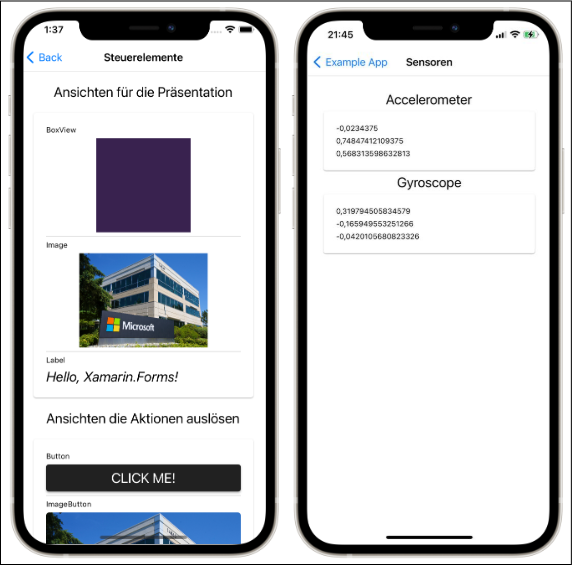
\includegraphics[width=\textwidth,keepaspectratio]{Images/Screenshot/Sensors.png}
 \caption{Test Objekt Screenshots II}
 \label{fig:TestObjectII}
\end{figure}

\section{Testfälle}
Um den Compiler zu Testen ist es notwendig Testfälle zu definieren und zu überprüfen, ob der Compiler die Xamarin.Forms App so übersetzt, wie es zu erwarten.   Zu diesem Zweck werden in diesem Abschnitt Testfälle definiert die sich aus den ermittelten Unterschieden zwischen beiden Frameworks,  sowie der Programmiersprachen ergeben.  Tabelle \ref{tab:Testapp} beschreibt die Testfälle und ihre entsprechenden Funktionen.


\begin{xltabular}{\textwidth}{l|l|X}
   \textbf{ID} & \textbf{Komponente} & \textbf{Beschreibung}  \\  


\hline
1             & App-Icon           	& Prüfen ob das App-Icon übernommen wurde                      			 \\ 
2             & App-Name          	& Prüfen ob das App-Name übernommen wurde                      		 \\ 
3             & SDK Versionen      & Prüfen ob die SDK Versionen übernommen wurden                      \\ 
4             & Seitenname           				& In der Navigationsleiste wird der Name der aktuellen Seite angezeigt               \\ 
5          	  & Navigation         			  	& Mit Hilfe des Menüs kann navigiert werden                      			 \\ 
6             & Zurück Navigation           	& Über die Navigationsleiste kann zurrück Navigiert werden                      			 \\ 
7             & Gyroscope auswerten           	& Die Werte werden in der App angezeigt.                      			 \\ 
8             & Accelerometer auswerten           	& Die Werte werden in der App angezeigt.                   			 \\ 
9             & Compass auswerten           	& Die Werte werden in der App angezeigt.                			 \\ 
10            & Magnetometer auswerten           	& Die Werte werden in der App angezeigt.                			 \\ 
11            & Sensor nicht verfügbar         	& Wenn ein Sensor nicht verfügbar ist, wird ein Fehler angezeigt          			 \\ 
12            & Steuerelemente 	           		& Alle Steuerelemente werden angezeigt        			 \\ 
13            & Ereignisse funktionieren           	&  Steuerelemente reagieren wie gewohnt     			 \\ 
14            & Bild aus Ressourcen laden           	& Ein Bild aus den Ressourcen wird in der App angezeigt                   			 \\ 
15             & Bild aus dem Web laden           	& Ein Bild aus dem Internet wird in der App                      			 \\ 

	  \caption{Testfälle der Testapp}

 \label{tab:Testapp}
\end{xltabular}


\section{Testablauf}
Der Start  des Testlaufs beginnt mit dem Aufruf der grafischen Benutzeroberfläche und der Auswahl sowohl der Xamarin.Forms Testapp, als auch eines leeren Ordners, der das Zielverzeichnis nach der Kompilierung dient. 
Aufgrund der vielen Dateizugriffe und durchzuführenden Aktionen nimmt die Übersetzung der Anwendung eine gewisse Zeit in Anspruch.  Im Frontend lassen sich Informationen bezüglich der Übersetzung ablesen, wenn sie erfolgreich absolviert wurde.  Anschließend kann die übersetzte Flutter Anwendung mithilfe der Flutter-SDK kompiliert und die übersetzten Ansichten kontrolliert werden.  Die folgenden Screenshots zeigen das Flutterergebnis. Die entsprechenden Screenshots von Android befinden sich im Anhang dieser Arbeit.

Die Screenshots zeigen,  auf den ersten Blick die erwartete visuelle Vergleichbarkeit der Anwendungen.  Sowohl der Name als auch das Launchericon der Anwendung sind korrekterweise übernommen worden.  Nach dem Start der Anwendung fällt auf,  dass die App etwas anders aussieht als die Xamarin.Forms iOS Anwendung.  Dies ist begründet durch die Verwendung der Material Design Vorlagen.  Da der Compiler, wie in den Ausschlusskriterien beschrieben nicht den Style der Anwendungen übersetzt ist dieses verhalten,  das erwartete und daher an dieser Stelle akzeptabel.  Das zentrale Menü der Anwendung ist auch in der Flutter Anwendung verfügbar und die Navigation über dieses funktioniert wie bei Xamarin.Forms ausschließlich die Animation ist unterschiedlich.  Die Ansicht der verfügbaren Ansichten zeigt, dass sowohl die Verschachtelung der Widgets als auch ihre Funktionalitäten mit der Xamarin.Forms Variante übereinstimmen.  So lassen sich beispielsweise auch die Datum- und Uhrzeitsauswahl öffnen. 
Die Ansicht der Sensoren zeigen,  dass auch hier die Oberfläche korrekt übernommen wurde und auch,  dass die Werte der Smartphone-Sensoren übernommen und im richtigen Format angezeigt sind.  Im Gegensatz zu Xamarin.Forms werden diese Daten jedoch nicht im gleichen zyklus aktualisiert.  Dieser Unterschied basiert auf den Implementationen des jeweiligen Plugins und entsteht nicht durch den Übersetzer.  Auch die Verwendung der Kamera und der Zugriff auf die Galerie funktionieren wie in der Xamarin.Forms Anwendung. 

Mit der im März 2021 veröffentlichten Version 2.0 von Flutter können Flutter Anwendungen ebenfalls zu Web-Anwendungen kompiliert werden.  Auch wenn die Erstellungen von Webseiten nicht im Fokus dieser Arbeit steht soll diese Anwendung trotzdem kurz betrachtet werden.  Die grundlegende Darstellung ist identisch wie die der mobilen Anwendung.  Da die Xamarin.Forms App nicht darauf ausgelegt war auch großen Monitoren dargestellt zu werden ist diese Ansicht zwar nicht für diese Darstellung optimiert aber funktionsfähig.  Die Funktionalitäten der Sensoren sind jedoch nicht Verfügbar, da das Plugin keinen Support für Flutter-Web bietet. 

\begin{figure}[!ht]
 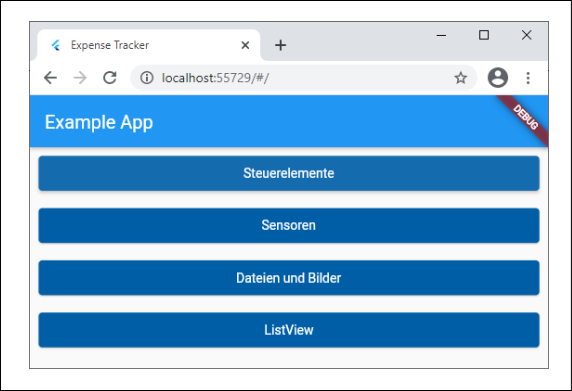
\includegraphics[width=\textwidth,keepaspectratio]{Images/Implementation/WebApp.png}
 \caption{Darstellung des Testobjektes als Webseite}
 \label{fig:WebView}
\end{figure}



Obwohl das Testobjekt nicht alle  Xamarin.Forms Funktionalitäten abbildet,  konnte das Testobjekt vollständig überführt und die Funktionsfähigkeit des Prototypen bewiesen werden.  

